# Details on implementation

The SDC scheduler with simulated annealing is implemented in the \code{SASDC}-class. The constructor takes the resource constraints and the scheduling quality as parameters. The quality is forwarded to the inner-loop-criterion, which is explained in chapter 3.\par
The actual implementation of the SA algorithm is straight forward, therefore the real point of interest is how the configuration for a schedule is created and how it can be modified with having the option to revert the modification. This is done with a helper class \code{SDCNodeList} (for the sake of simplicity furthermore just called "node list").\par
The node list basically takes the the graph to schedule as constructor parameter. Then it initializes a corresponding \code{Node}-array with a length equals to the number of nodes in the graph. The original \code{Node}-class (from the high-level-framework) has got a new parameter \code{depth}, which is the hierarchical depth of each node (i.e. root-nodes have depth=0, their predecessors have depth=1 and so on). The \code{Node}-array will then be filled ordered by the corresponding depths. This leads to the initial node list which then can be modified in order to optimize the results.\par
To get better results, the list must be reordered somehow, but it must not do "wild swapping" of nodes - the reordering is restricted by the data flow dependencies. To clear this up a bit, figure~\ref{fig:lecturegraph} shows the example graph from the lecture.
\begin{figure}
	\centering
	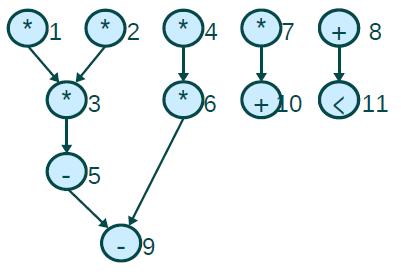
\includegraphics{lecturegraph.png}
	\caption{Example Graph (\cite{Hochberger2017}, Chapter 3, Slide 97)}
	\label{fig:lecturegraph}
\end{figure}

The initial order of the node list (due to the hierarchical depth) could be #1, #2, #4, #7, #8, #3, #6, #10, #11, #5, #9. Node #3 e.g. is a data flow dependency of #1, #2, #5 and #9. Exactly these dependencies must be considered when #3 is moved in the list. To be more precise, each predecessor of #3 must always be left of #3 and each successor must always be to the right. This restricts the degree of flexibility when modifying the list.\\
To make modification easy, the \code{SDCNodeList} provides two methods \code{shoveRight} and \code{shoveLeft}, which do the following:

%
% BITTE PSEUDOCODE DRAUS MACHEN (KANNS BEI MIR NICHT TESTEN)
%
shoveRight(i0: int):
	// nodes is a class-member
	shoveCount: int
	for(int i := i0+1; i < nodes.length; i++)
		// find first non-flow-dependend-node
		if (nodes[i] isNoSuccessorOf nodes[i0])
			shoveCount = i - i0;
			break;

	// move items  [i0 ... i0 + shoveCount] one array i0 to the right
	// set original item from list[i0] = list[i0 + shoveCount]

This is a generic example and works in almost the same manner for shoveLeft. Basically the shove-functions find the first non-dependend predecessor/successor node beginning searching at \code{i0}. The initial ordering in the example before ended with the nodes #11, #5, #9. When shoving #9 to the left, the first node which would be checked to be predecessor is #5. Next iteration, #11 fulfils the \textit{isNoPredecessor}-criterion, therefore the \code{shoveCount} would be set to 2 and the loop cancels. Now the elements would be reordered to #5, #9, #11.\par
By storing the \code{i0} and \code{shoveCount}, the operation can easily be reverted if the change is not accepted the SA algorithm.
	
